\chapter{Symmetry and Point Groups}\label{ch:b3:point-groups}

Turn a snowflake by sixty degrees and nothing changes; turn a benzene
molecule by the same angle, and its six carbons and six hydrogens fall
exactly on each other's places. The symmetry of a molecule decides several
of its properties before any calculation: whether it can have a dipole
moment, whether it can exist as two mirror-image forms, which of its
vibrations absorb infrared light, which orbitals may mix. To use it, chemists
borrowed from mathematics the language of groups. This chapter defines the
\omterm{def:b3:point-groups:operation}{symmetry operations} of a molecule, collects them into its \omterm{def:b3:point-groups:point-group}{point group},
gives a procedure to find that group, proves two theorems on polarity and
chirality, and introduces the \omterm{def:b3:point-groups:irrep}{character tables} on which
\cref{ch:b3:group-theory-applied} builds.

\begin{recall}
The Year 1 volume predicted molecular shapes with the VSEPR model, defined
the dipole moment of a polar molecule, and defined chirality: a chiral
molecule cannot be superimposed on its mirror image. The Year 2 volume used
symmetry in words to build the fragment orbitals of \ce{H2O} and \ce{NH3}.
\end{recall}

\begin{omfigure}
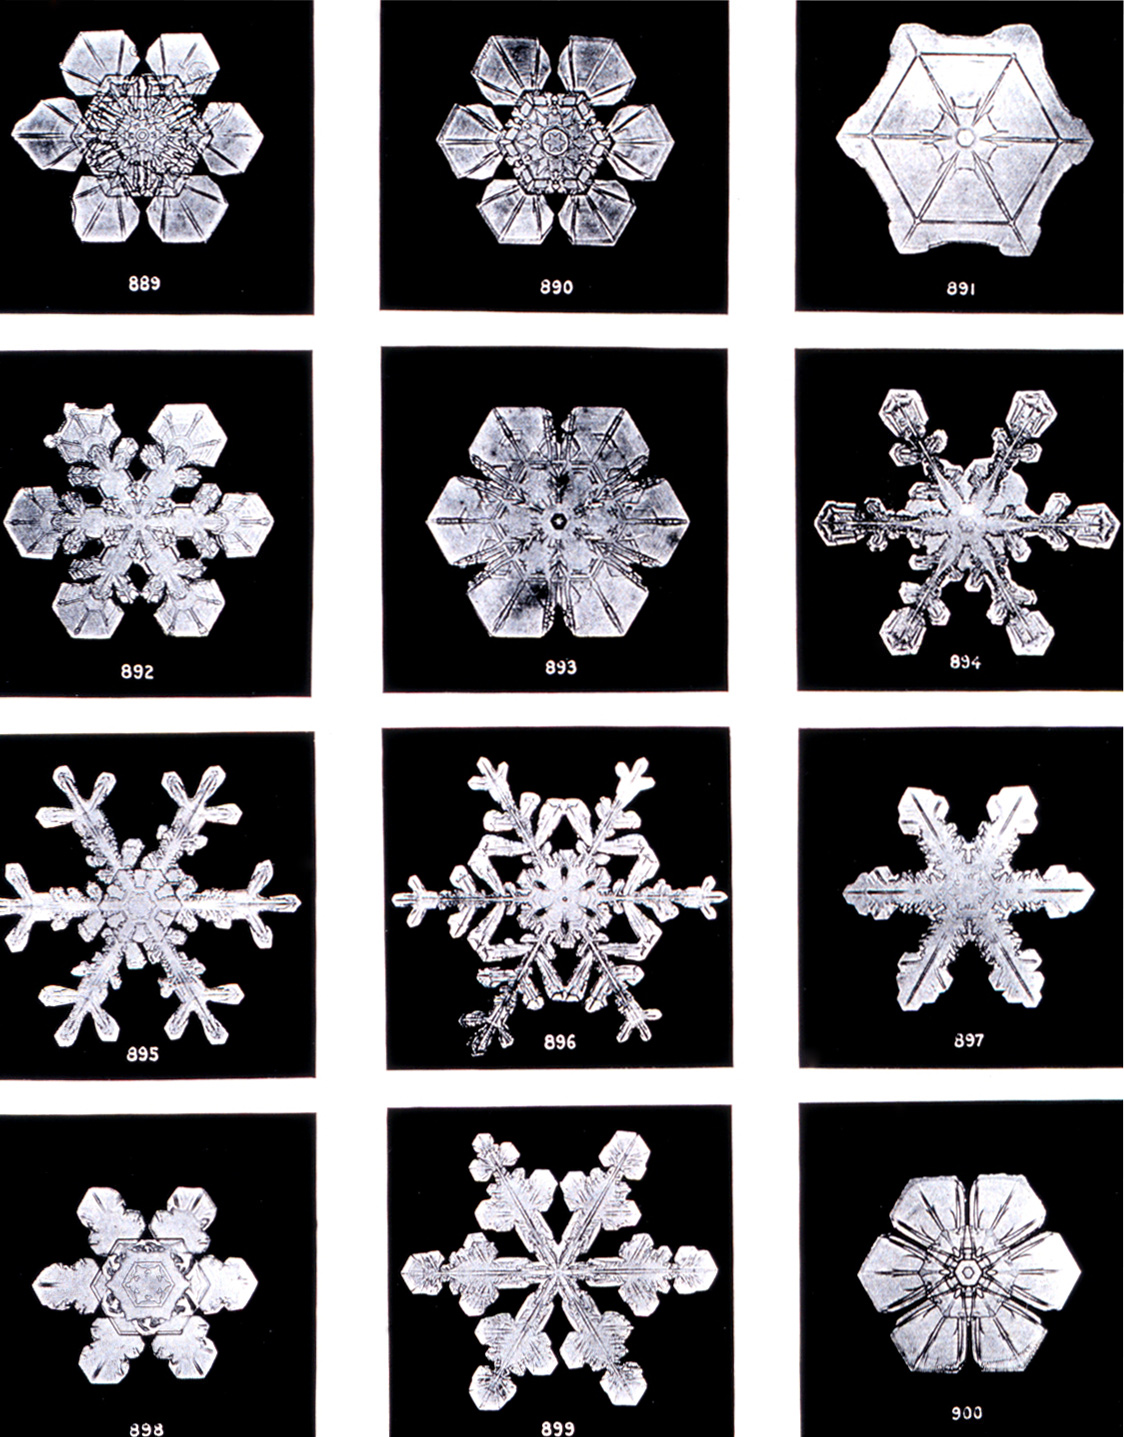
\includegraphics[width=0.4\linewidth]{images/book4/bentley-snowflakes.jpg}\hspace{1em}%
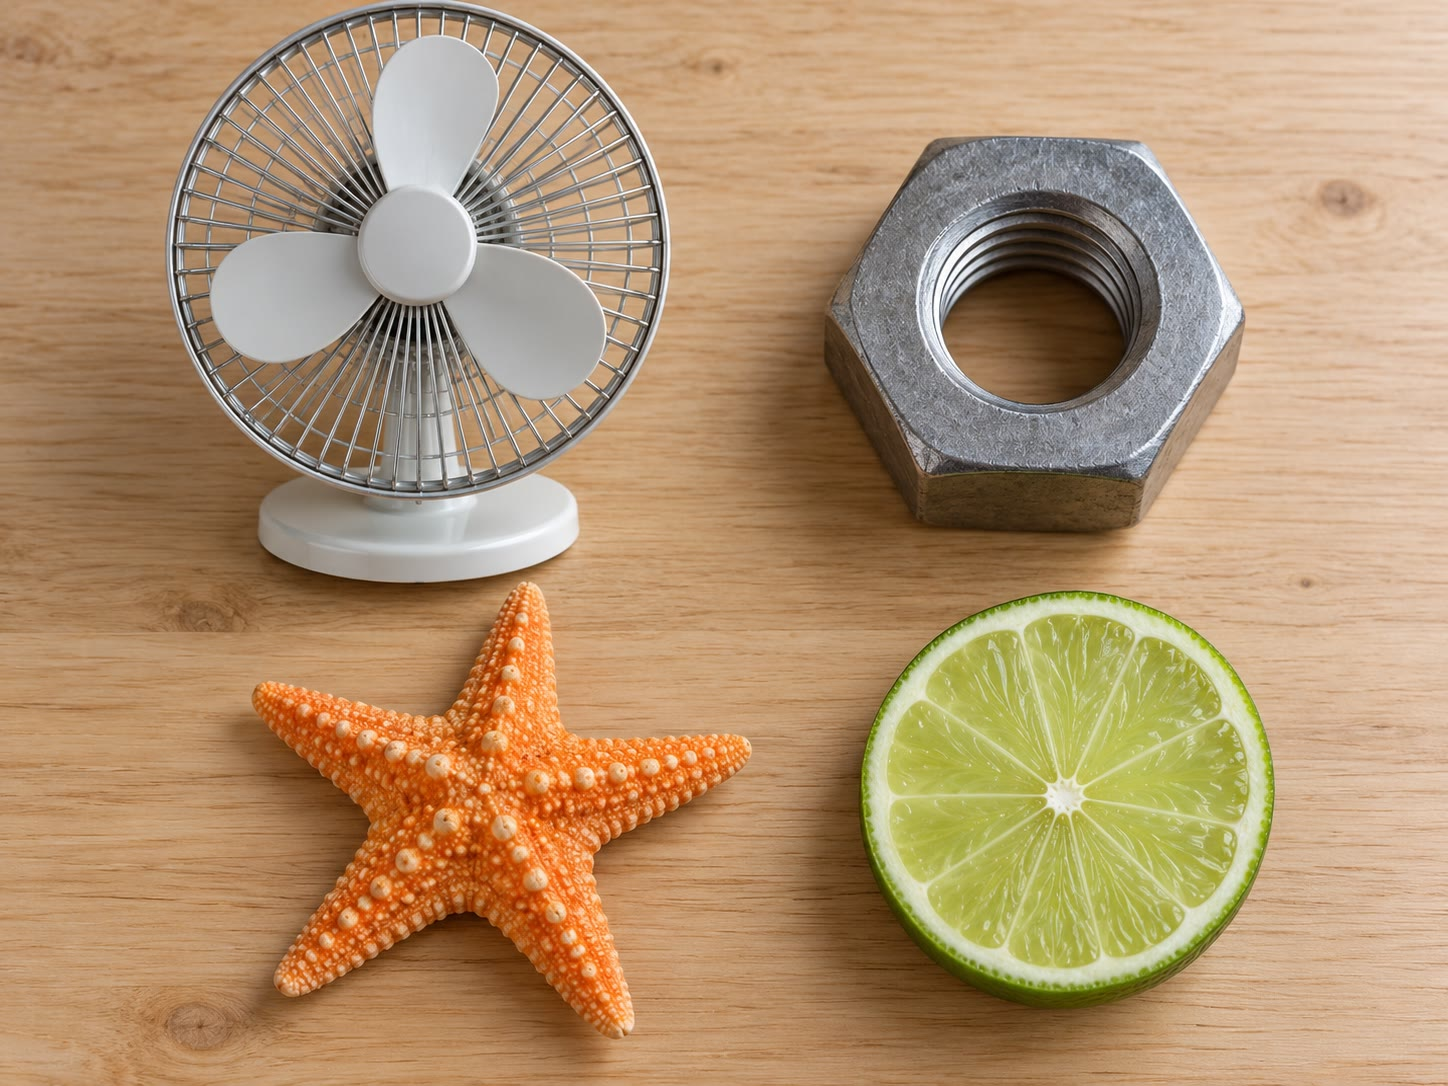
\includegraphics[width=0.48\linewidth]{images/book4/ai/b3-04-symmetric-objects.jpg}

{\small Left: snow crystals photographed by Wilson Bentley around 1902,
each with sixfold symmetry. Right: everyday objects with threefold, sixfold
and fivefold rotational symmetry.}
\end{omfigure}

\section{Symmetry operations and elements}

\begin{definition}[Symmetry operation, symmetry element]\label{def:b3:point-groups:operation}
A \emph{symmetry operation}\index{symmetry operation} is a motion or
reflection that leaves a molecule in a configuration indistinguishable from
the original (each atom on a position occupied before by an atom of the same
kind). A \emph{symmetry element}\index{symmetry element} is the geometric
object --- a point, a line, a plane --- with respect to which the operation
is performed.
\end{definition}

Every molecule has the identity operation $E$, which does nothing. The
others come in four kinds.

\begin{definition}[Proper rotation axis, principal axis]\label{def:b3:point-groups:rotation}
A \emph{proper rotation axis}\index{proper rotation axis} $C_n$ is a line
about which a rotation by $2\pi/n$ is a \omterm{def:b3:point-groups:operation}{symmetry operation}, also written
$C_n$; its powers $C_n^k$ are rotations by $2\pi k/n$, and $C_n^n = E$. The
axis of highest $n$ is the \emph{principal axis}\index{principal axis}, taken
as $z$.
\end{definition}

\begin{definition}[Mirror planes]\label{def:b3:point-groups:mirror}
A \emph{mirror plane}\index{mirror plane} $\sigma$ is a plane through which
reflection is a \omterm{def:b3:point-groups:operation}{symmetry operation}; $\sigma^2 = E$. A mirror plane is a
\emph{vertical mirror plane}\index{vertical mirror plane} $\sigma_v$ if it
contains the \omterm{def:b3:point-groups:rotation}{principal axis}, a \emph{horizontal mirror
plane}\index{horizontal mirror plane} $\sigma_h$ if it is perpendicular to
it, and a \emph{dihedral mirror plane}\index{dihedral mirror plane}
$\sigma_d$ if it contains the \omterm{def:b3:point-groups:rotation}{principal axis} and bisects the angle between
two $C_2$ axes perpendicular to it.
\end{definition}

\begin{definition}[Centre of inversion]\label{def:b3:point-groups:inversion}
A \emph{centre of inversion}\index{centre of inversion} $i$ is a point
through which inversion, $(x, y, z) \mapsto (-x, -y, -z)$, is a \omterm{def:b3:point-groups:operation}{symmetry
operation}.
\end{definition}

\begin{definition}[Improper rotation axis]\label{def:b3:point-groups:improper}
An \emph{improper rotation axis}\index{improper rotation axis} $S_n$ is a
line about which a rotation by $2\pi/n$ followed by reflection in the plane
perpendicular to it is a \omterm{def:b3:point-groups:operation}{symmetry operation}. $S_1 = \sigma$ and $S_2 = i$.
\end{definition}

\begin{example}[Elements of four molecules]\label{ex:b3:point-groups:elements}
\ce{H2O}: $E$, a $C_2$ axis bisecting the H--O--H angle, and two vertical
planes, the molecular plane and the plane perpendicular to it. \ce{NH3}:
$E$, a $C_3$ through N (operations $C_3$ and $C_3^2$), and three $\sigma_v$, each
containing one N--H bond. \ce{BF3}: a $C_3$, three $C_2$ along the B--F bonds,
$\sigma_h$ (the molecular plane), three $\sigma_v$, and an $S_3$. \ce{CH4}: four
$C_3$ along the C--H bonds, three $C_2$ bisecting H--C--H angles, which are
also $S_4$ axes, and six $\sigma_d$, each containing two C--H bonds
(figure below).
\end{example}

\begin{omfigure}
\begin{tikzpicture}[font=\small]
  % H2O, side view: molecular plane xz (shaded), C2 along z
  \begin{scope}
    \fill[omDef!10] (-1.5,-1.0) -- (1.5,-1.0) -- (1.5,1.2) -- (-1.5,1.2) -- cycle;
    \fill[omThm!12, opacity=0.8] (-0.45,-1.35) -- (0.45,-0.65) -- (0.45,1.55) -- (-0.45,0.85) -- cycle;
    \draw[densely dashed, black!70] (0,-1.4) -- (0,1.7) node[above] {$C_2$};
    \node[aO] (o) at (0,0.5) {};
    \node[aH] (h1) at (-0.95,-0.25) {};
    \node[aH] (h2) at (0.95,-0.25) {};
    \begin{scope}[on background layer]
      \draw[bond] (o.center) -- (h1.center) (o.center) -- (h2.center);
    \end{scope}
    \node[omDef, anchor=north west] at (-1.5,1.2) {$\sigma_v(xz)$};
    \node[omThm, anchor=west] at (0.5,-0.85) {$\sigma_v'(yz)$};
    \node[anchor=north] at (0,-1.6) {\ce{H2O}, $C_{2v}$};
  \end{scope}
  % NH3, top view along C3
  \begin{scope}[xshift=4.0cm]
    \foreach \a in {90,210,330}{\draw[ommirror] (0,0) -- (\a:1.35); \draw[ommirror, black!40] (0,0) -- (\a+180:1.0);}
    \foreach \a in {90,210,330}{\node[aH] at (\a:0.95) {};}
    \node[aN] at (0,0) {};
    \pic at (0,0) {omthreefold};
    \node[anchor=north] at (0,-1.6) {\ce{NH3}, $C_{3v}$ (from above)};
  \end{scope}
  % BF3, top view; sigma_h = plane of the paper (thick circle)
  \begin{scope}[xshift=8.0cm]
    \draw[ommirror] (0,0) circle (1.3);
    \foreach \a in {90,210,330}{\draw[ommirror] (\a:1.3) -- (\a+180:1.3);}
    \foreach \a in {90,210,330}{\pic[rotate=\a-90] at (\a:1.42) {omtwofold}; \pic[rotate=\a-90] at (\a+180:1.42) {omtwofold};}
    \foreach \a in {90,210,330}{\node[aF] at (\a:0.95) {};}
    \node[aX={pink!70!gray}{5.6mm}] at (0,0) {};
    \pic at (0,0) {omthreefold};
    \node[anchor=north] at (0,-1.6) {\ce{BF3}, $D_{3h}$ (from above)};
  \end{scope}
\end{tikzpicture}

{\small \omterm{def:b3:point-groups:operation}{Symmetry elements}. \ce{H2O}: the $C_2$ axis (dashed) and two \omterm{def:b3:point-groups:mirror}{vertical
mirror planes}. \ce{NH3} and \ce{BF3} seen down their \omterm{def:b3:point-groups:rotation}{principal axis} (triangle
glyph): thick lines are \omterm{def:b3:point-groups:mirror}{mirror planes} seen edge-on; in \ce{BF3} the thick
circle marks the \omterm{def:b3:point-groups:mirror}{horizontal mirror plane} (the plane of the page) and the
lens glyphs the three $C_2$ axes lying in it.}
\end{omfigure}

\section{Groups}

\begin{proposition}[Products of symmetry operations]\label{prop:b3:point-groups:closure}
Performing two \omterm{def:b3:point-groups:operation}{symmetry operations} of a molecule in succession is again a
\omterm{def:b3:point-groups:operation}{symmetry operation} of that molecule. Together with $E$ and the inverse of
each operation, the set of \omterm{def:b3:point-groups:operation}{symmetry operations} is a group: an associative
product, an identity, an inverse for each element.
\end{proposition}

\begin{proof}
Each operation leaves the molecule indistinguishable from itself, so two in
succession do too. The product of operations (composition of maps of space)
is associative; $E$ is the identity; an operation undone (a rotation by the
opposite angle, a reflection repeated) is also a \omterm{def:b3:point-groups:operation}{symmetry operation}.
\end{proof}

\begin{proposition}[A common point]\label{prop:b3:point-groups:fixed-point}
All the \omterm{def:b3:point-groups:operation}{symmetry elements} of a finite molecule pass through one point.
\end{proposition}

\begin{proof}
Every \omterm{def:b3:point-groups:operation}{symmetry operation} maps each atom onto an atom of the same mass, so it
leaves the centre of mass unchanged. A rotation fixes only the points of its
axis, a reflection those of its plane, an improper rotation or an inversion
a single point: every element contains the centre of mass.
\end{proof}

\begin{definition}[Point group, order of a point group]\label{def:b3:point-groups:point-group}
The group of all \omterm{def:b3:point-groups:operation}{symmetry operations} of a molecule is its \emph{point
group}\index{point group}, named because one point stays fixed. The number of
its operations is the \emph{order of a point group}\index{order of a point group},
$h$.
\end{definition}

\begin{example}[The group of water]\label{ex:b3:point-groups:c2v}
The four operations $E$, $C_2$, $\sigma_v(xz)$, $\sigma_v'(yz)$ of \ce{H2O} form a
group of order 4. Its multiplication table (row operation performed after the
column one) is
\begin{center}\small
\begin{tabular}{c|cccc}
\hline
 & $E$ & $C_2$ & $\sigma_v(xz)$ & $\sigma_v'(yz)$\\ \hline
$E$ & $E$ & $C_2$ & $\sigma_v(xz)$ & $\sigma_v'(yz)$\\
$C_2$ & $C_2$ & $E$ & $\sigma_v'(yz)$ & $\sigma_v(xz)$\\
$\sigma_v(xz)$ & $\sigma_v(xz)$ & $\sigma_v'(yz)$ & $E$ & $C_2$\\
$\sigma_v'(yz)$ & $\sigma_v'(yz)$ & $\sigma_v(xz)$ & $C_2$ & $E$\\ \hline
\end{tabular}
\end{center}
For instance a point $(x, y, z)$ reflected in $xz$ goes to $(x, -y, z)$, then
rotated by $\pi$ about $z$ to $(-x, y, z)$: the same as one reflection in
$yz$.
\end{example}

\begin{definition}[Class of symmetry operations, subgroup]\label{def:b3:point-groups:class}
Two operations $A$ and $B$ belong to the same \emph{class of symmetry
operations}\index{class of symmetry operations} if $B = X^{-1}AX$ for some
operation $X$ of the group: they are the same kind of operation, seen in a
frame moved by $X$. A subset of a group that is a group on its own is a
\emph{subgroup}\index{subgroup}; its order divides the order of the group.
\end{definition}

\begin{example}[Classes of \ce{NH3}]\label{ex:b3:point-groups:classes}
In $C_{3v}$ ($h = 6$), the three reflections form one class (a $C_3$ rotation
carries each plane onto another), the two rotations $C_3$ and $C_3^2$ another,
and $E$ is a class alone: three classes, written $E$, $2C_3$, $3\sigma_v$. In
$C_{2v}$ every operation is its own class: no operation turns one plane into
the other.
\end{example}

\begin{definition}[Schoenflies symbol]\label{def:b3:point-groups:schoenflies}
A \omterm{def:b3:point-groups:point-group}{point group} is named by its \emph{Schoenflies symbol}\index{Schoenflies symbol}:
$C_n$ (one $C_n$ axis), $C_{nv}$ (adding $n$ vertical planes), $C_{nh}$
(adding $\sigma_h$), $D_n$ (adding $n$ $C_2$ axes perpendicular to $C_n$), $D_{nh}$
and $D_{nd}$ (adding $\sigma_h$, or $n$ dihedral planes, to $D_n$), $S_{2n}$, the
cubic groups $T_d$, $O_h$, $I_h$ of the tetrahedron, octahedron and
icosahedron, and $C_s$, $C_i$, $C_1$ for molecules with only a \omterm{def:b3:point-groups:mirror}{mirror plane},
only an inversion centre, or nothing at all. Linear molecules belong to
$C_{\infty v}$ or $D_{\infty h}$.
\end{definition}

\section{Assigning a point group}

\begin{method}[Finding the point group of a molecule]\label{met:b3:point-groups:assign}
\begin{enumerate}
  \item Is the molecule linear? With an inversion centre, $D_{\infty h}$
        (\ce{CO2}, \ce{N2}); without, $C_{\infty v}$ (\ce{HCl}, \ce{HCN}).
  \item Does it have several high-order axes ($n \ge 3$)? Tetrahedral shape:
        $T_d$; octahedral: $O_h$; icosahedral: $I_h$.
  \item Find the \omterm{def:b3:point-groups:rotation}{principal axis} $C_n$ (none: $C_s$ if a plane, $C_i$ if a
        centre, $C_1$ otherwise).
  \item Are there $n$ $C_2$ axes perpendicular to $C_n$? If yes, the group is
        $D_{nh}$ (with $\sigma_h$), else $D_{nd}$ (with $n$ $\sigma_d$), else
        $D_n$.
  \item If no: $C_{nh}$ (with $\sigma_h$), $C_{nv}$ (with $n$ $\sigma_v$), $S_{2n}$
        (with only an $S_{2n}$ collinear with $C_n$), else $C_n$.
\end{enumerate}
\end{method}

\begin{omfigure}
\begin{tikzpicture}[font=\footnotesize, node distance=6mm and 11mm,
  q/.style={draw=black!60, fill=omDef!6, rounded corners=2pt, align=center, inner sep=3pt},
  g/.style={draw=black!60, fill=omProp!10, rounded corners=2pt, inner sep=3pt}]
  \node[q] (lin) {linear?};
  \node[g, right=of lin] (dinf) {$D_{\infty h}$ / $C_{\infty v}$ (with / without $i$)};
  \node[q, below=of lin] (cub) {two or more $C_n$, $n \ge 3$?};
  \node[g, right=of cub] (td) {$T_d$, $O_h$, $I_h$};
  \node[q, below=of cub] (cn) {a $C_n$ axis?};
  \node[g, right=of cn] (low) {$C_s$, $C_i$ or $C_1$ (no)};
  \node[q, below=of cn] (c2) {$n$ $C_2 \perp C_n$?};
  \node[q, right=of c2, xshift=6mm] (dh) {$\sigma_h$?\; else $n$ $\sigma_d$?};
  \node[g, right=of dh] (dg) {$D_{nh}$ / $D_{nd}$ / $D_n$};
  \node[q, below=of c2] (sh) {$\sigma_h$?\; else $n$ $\sigma_v$?\; else $S_{2n}$?};
  \node[g, right=of sh] (cg) {$C_{nh}$ / $C_{nv}$ / $S_{2n}$ / $C_n$};
  \draw[->] (lin) -- node[above] {yes} (dinf);
  \draw[->] (lin) -- node[left] {no} (cub);
  \draw[->] (cub) -- node[above] {yes} (td);
  \draw[->] (cub) -- node[left] {no} (cn);
  \draw[->] (cn) -- node[above] {no} (low);
  \draw[->] (cn) -- node[left] {yes} (c2);
  \draw[->] (c2) -- node[above] {yes} (dh);
  \draw[->] (dh) -- (dg);
  \draw[->] (c2) -- node[left] {no} (sh);
  \draw[->] (sh) -- (cg);
\end{tikzpicture}

{\small The search for a \omterm{def:b3:point-groups:point-group}{point group}, in the order of the method.}
\end{omfigure}

\begin{example}[A gallery]\label{ex:b3:point-groups:gallery}
\ce{H2O}, \ce{CH2Cl2}, \ce{SO2}: $C_{2v}$. \ce{NH3}, \ce{CHCl3}: $C_{3v}$. \ce{BF3},
\ce{PCl5}: $D_{3h}$. \ce{CH4}, \ce{CCl4}: $T_d$. \ce{SF6}: $O_h$. Benzene: $D_{6h}$.
Ethene: $D_{2h}$. Ethane: $D_{3d}$ staggered, $D_{3h}$ eclipsed. Allene
\ce{H2C=C=CH2}: $D_{2d}$, the two \ce{CH2} planes at right angles. Cyclohexane
in its chair: $D_{3d}$. trans-\ce{N2F2}: $C_{2h}$. \ce{CHFClBr}: $C_1$.
\end{example}

\begin{omfigure}
\tdplotsetmaincoords{60}{100}
\begin{tikzpicture}[tdplot_main_coords, scale=1.6, font=\small]
  \pic[transform shape] {omcubeo={2}};
  % depth order for view 60/100 (smallest first): H(0,0,0), H(0,2,2), C, H(2,2,0), H(2,0,2)
  \draw[densely dashed, omThm, thick] (-0.4,-0.4,-0.4) -- (2.5,2.5,2.5) node[anchor=south west] {$C_3$};
  \draw[densely dashed, omDef, thick] (1,1,-0.5) -- (1,1,2.6) node[anchor=south] {$S_4$, $C_2$};
  \node[aH] (h1) at (0,0,0) {};
  \node[aH] (h4) at (0,2,2) {};
  \node[aC] (c) at (1,1,1) {};
  \node[aH] (h2) at (2,2,0) {};
  \node[aH] (h3) at (2,0,2) {};
  \begin{scope}[on background layer]
    \draw[bond] (c.center) -- (h1.center) (c.center) -- (h2.center)
                (c.center) -- (h3.center) (c.center) -- (h4.center);
  \end{scope}
\end{tikzpicture}

{\small Methane in a cube, its carbon at the centre and its hydrogens on
alternate corners. A body diagonal through one hydrogen is a $C_3$ axis
(four of them); the axis through two opposite face centres is a $C_2$ and an
$S_4$ axis (three of them). The \omterm{def:b3:point-groups:point-group}{point group} is $T_d$, of order 24.}
\end{omfigure}

\section{Consequences: polarity and chirality}

\begin{theorem}[Polar molecules]\label{thm:b3:point-groups:polar}
A molecule can have a permanent dipole moment only if its \omterm{def:b3:point-groups:point-group}{point group} is
$C_1$, $C_s$, $C_n$ or $C_{nv}$; the dipole then lies along the \omterm{def:b3:point-groups:rotation}{principal axis}
(in the plane, for $C_s$).
\end{theorem}

\begin{proof}
The dipole moment is a vector property of the molecule, so every \omterm{def:b3:point-groups:operation}{symmetry
operation} must leave it unchanged. A rotation about an axis leaves only
vectors along that axis unchanged; two axes leave no non-zero vector; a
$\sigma_h$, an $i$ or an $S_n$ reverses any vector along the axis; a $\sigma_v$
keeps vectors in its plane. Hence a non-zero dipole requires at most one
axis, no $\sigma_h$, no $i$, no $S_n$: the groups listed.
\end{proof}

\begin{example}[Polar or not]\label{ex:b3:point-groups:polar}
\ce{H2O}, \ce{NH3}, \ce{CHCl3} and \ce{SO2} ($C_{2v}$, $C_{3v}$) can be polar, and
are. \ce{BF3} ($D_{3h}$), \ce{CO2} ($D_{\infty h}$), \ce{CH4} ($T_d$), \ce{SF6} ($O_h$)
and trans-\ce{N2F2} ($C_{2h}$) cannot, whatever their polar bonds.
\end{example}

\begin{theorem}[Chiral molecules]\label{thm:b3:point-groups:chiral}
A molecule is chiral if and only if it has no \omterm{def:b3:point-groups:improper}{improper rotation axis} $S_n$
(including $S_1 = \sigma$ and $S_2 = i$).
\end{theorem}

\begin{proof}
If the molecule has an $S_n$, then $S_n = \sigma_hC_n$: the mirror image $\sigma_h$
of the molecule equals $C_n^{-1}$ applied to the molecule after $S_n$, that is
the molecule rotated --- superimposable, hence achiral. Conversely, if the
molecule is achiral, its mirror image $\sigma M$ can be brought onto $M$ by a
proper motion $R$ (a rotation about the centre of mass): $R\sigma$ is then a
\omterm{def:b3:point-groups:operation}{symmetry operation}. It is improper (it changes handedness, its matrix has
determinant $-1$), and every improper operation of a \omterm{def:b3:point-groups:point-group}{point group} is an
$S_n$ for some $n$ (a rotation followed by a reflection in the perpendicular
plane). So the molecule has an $S_n$.
\end{proof}

\begin{example}[An achiral molecule without a plane]\label{ex:b3:point-groups:s4}
Some molecules have neither a \omterm{def:b3:point-groups:mirror}{mirror plane} nor a \omterm{def:b3:point-groups:inversion}{centre of inversion}, yet
are achiral because of an $S_4$ axis: the classic case is a spiro compound
built from two identically substituted rings at right angles, of \omterm{def:b3:point-groups:point-group}{point
group} $S_4$. Chirality cannot be judged by looking for a plane alone.
\end{example}

\section{Representations and character tables}

Each \omterm{def:b3:point-groups:operation}{symmetry operation} moves a point $(x, y, z)$ linearly: it can be written
as a $3\times3$ matrix.

\begin{definition}[Matrix representation, character]\label{def:b3:point-groups:representation}
A \emph{matrix representation}\index{matrix representation} $\Gamma$ of a
\omterm{def:b3:point-groups:point-group}{point group} assigns to each operation $R$ a square matrix $D(R)$ such that
$D(R_1R_2) = D(R_1)D(R_2)$: products of operations become products of
matrices. The \emph{character}\index{character} $\chi(R)$ of $R$ in $\Gamma$ is
the trace of $D(R)$.
\end{definition}

\begin{example}[The coordinates of $C_{3v}$]\label{ex:b3:point-groups:xyz}
For $C_3$ about $z$, $D = \begin{psmallmatrix}\cos120^\circ & -\sin120^\circ &
0\\ \sin120^\circ & \cos120^\circ & 0\\ 0 & 0 & 1\end{psmallmatrix}$, of trace
$2\cos120^\circ + 1 = 0$; for $\sigma_v(xz)$, $D = \mathrm{diag}(1, -1, 1)$, trace
1; for $E$, trace 3. The \omterm{def:b3:point-groups:representation}{characters} of this representation are $(3, 0, 1)$ on
the classes $(E, 2C_3, 3\sigma_v)$. Every matrix is block-diagonal, a
$2\times2$ block for $(x, y)$ and a $1\times1$ block for $z$: the
representation splits into two smaller ones.
\end{example}

\begin{proposition}[Characters are class functions]\label{prop:b3:point-groups:class-characters}
Operations of the same class have the same \omterm{def:b3:point-groups:representation}{character} in any representation.
\end{proposition}

\begin{proof}
If $B = X^{-1}AX$, then $D(B) = D(X)^{-1}D(A)D(X)$, and the trace is unchanged by
such a change of basis: $\mathrm{tr}(P^{-1}MP) = \mathrm{tr}(M)$.
\end{proof}

\begin{proposition}[Reducing by blocks]\label{prop:b3:point-groups:direct-sum}
If a basis can be split into subsets that every operation maps into
themselves, all matrices are block-diagonal, and the representation is the
sum of the smaller representations carried by the subsets; its \omterm{def:b3:point-groups:representation}{characters}
are the sums of theirs.
\end{proposition}

\begin{proof}
An operation that maps each subset into itself has no matrix elements
between different subsets; the trace of a block-diagonal matrix is the sum
of the traces of its blocks.
\end{proof}

\begin{definition}[Irreducible representation, character table, Mulliken symbol]\label{def:b3:point-groups:irrep}
A representation that cannot be split further by any change of basis is an
\emph{irreducible representation}\index{irreducible representation}. The
\emph{character table}\index{character table} of a \omterm{def:b3:point-groups:point-group}{point group} lists the
\omterm{def:b3:point-groups:representation}{characters} of its irreducible representations, one row each, on its classes,
one column each, with the Cartesian functions and rotations that transform
like each row. The rows are named by their \emph{Mulliken
symbol}\index{Mulliken symbol}: $A$ or $B$ for one dimension (symmetric or
antisymmetric under the principal rotation), $E$ for two, $T$ for three;
subscripts 1, 2 (symmetric or antisymmetric under a $C_2$ or $\sigma_v$), $g$, $u$
(under inversion), primes (under $\sigma_h$).
\end{definition}

\begin{proposition}[Size of a character table]\label{prop:b3:point-groups:irrep-count}
A \omterm{def:b3:point-groups:point-group}{point group} has as many \omterm{def:b3:point-groups:irrep}{irreducible representations} as classes, and the
squares of their dimensions add up to the order: $\sum_id_i^2 = h$.
\end{proposition}
\begin{proof}[Status]
Proved in \cref{ch:b3:group-theory-applied} from the orthogonality of
\omterm{def:b3:point-groups:representation}{characters}, itself admitted there.
\end{proof}

% ledger: ct:C2v, ct:C3v, ct:Td
The tables needed most often in this book are those of water, ammonia and
methane:
\begin{omchartable}{C_{2v}}{cccc}{E & C_2 & \sigma_v(xz) & \sigma_v'(yz)}
A_1 & 1 & 1 & 1 & 1 & z & x^2,\ y^2,\ z^2 \\
A_2 & 1 & 1 & -1 & -1 & R_z & xy \\
B_1 & 1 & -1 & 1 & -1 & x,\ R_y & xz \\
B_2 & 1 & -1 & -1 & 1 & y,\ R_x & yz \\
\end{omchartable}
\begin{omchartable}{C_{3v}}{ccc}{E & 2C_3 & 3\sigma_v}
A_1 & 1 & 1 & 1 & z & x^2 + y^2,\ z^2 \\
A_2 & 1 & 1 & -1 & R_z & \\
E & 2 & -1 & 0 & (x, y),\ (R_x, R_y) & (x^2 - y^2, xy),\ (xz, yz) \\
\end{omchartable}
\begin{omchartable}{T_d}{ccccc}{E & 8C_3 & 3C_2 & 6S_4 & 6\sigma_d}
A_1 & 1 & 1 & 1 & 1 & 1 & & x^2 + y^2 + z^2 \\
A_2 & 1 & 1 & 1 & -1 & -1 & & \\
E & 2 & -1 & 2 & 0 & 0 & & (2z^2 - x^2 - y^2,\ x^2 - y^2) \\
T_1 & 3 & 0 & -1 & 1 & -1 & (R_x, R_y, R_z) & \\
T_2 & 3 & 0 & -1 & -1 & 1 & (x, y, z) & (xy, xz, yz) \\
\end{omchartable}

\begin{method}[Reading a character table]\label{met:b3:point-groups:matrices}
\begin{enumerate}
  \item The first column of \omterm{def:b3:point-groups:representation}{characters} (under $E$) is the dimension: the
        \omterm{def:b3:quantum-model-systems:degenerate}{degeneracy} of the levels or orbitals labelled by that row.
  \item A \omterm{def:b3:point-groups:representation}{character} $+1$ means the function is unchanged by the operation,
        $-1$ that it changes sign; a 0 in a degenerate row means the members
        of the set are mixed.
  \item To find how a function transforms, apply each operation to it and
        compare with the rows; the right-hand columns give the answer for
        $x$, $y$, $z$, the rotations, and the quadratic functions (the shapes
        of $d$ orbitals).
\end{enumerate}
\end{method}

\begin{example}[The orbitals of oxygen in water]\label{ex:b3:point-groups:water-orbitals}
In $C_{2v}$, the $2s$ and $2p_z$ orbitals of oxygen are unchanged by every
operation: $a_1$ (lower-case for orbitals). $2p_x$ changes sign under $C_2$ and
$\sigma_v'(yz)$: $b_1$. $2p_y$: $b_2$. These are the labels used for the water
orbitals in the Year 2 volume; \cref{ch:b3:group-theory-applied} derives the
labels of the hydrogen combinations.
\end{example}

\begin{omfigure}
\begin{tikzpicture}[font=\small]
  \begin{scope}
    \pic {omstereo={1.2}};
    \draw[ommirror] (-1.2,0) -- (1.2,0);
    \draw[ommirror] (0,-1.2) -- (0,1.2);
    \pic at (0,0) {omtwofold};
    \foreach \x/\y in {0.55/0.45,-0.55/0.45,0.55/-0.45,-0.55/-0.45}{\pic at (\x,\y) {omup};}
    \node[anchor=north] at (0,-1.35) {$C_{2v}$};
  \end{scope}
  \begin{scope}[xshift=4cm]
    \pic {omstereo={1.2}};
    \foreach \a in {90,210,330}{\draw[ommirror] (\a:1.2) -- (\a+180:1.2);}
    \pic at (0,0) {omthreefold};
    \foreach \a in {70,110,190,230,310,350}{\pic at (\a:0.75) {omup};}
    \node[anchor=north] at (0,-1.35) {$C_{3v}$};
  \end{scope}
  \begin{scope}[xshift=8cm]
    \pic {omstereo={1.2}};
    \draw[ommirror] (0,0) circle (1.2);
    \foreach \a in {90,210,330}{\draw[ommirror] (\a:1.2) -- (\a+180:1.2);}
    \pic at (0,0) {omthreefold};
    \foreach \a in {70,110,190,230,310,350}{\pic at (\a:0.75) {omup}; \pic at (\a:0.75) {omdown};}
    \node[anchor=north] at (0,-1.35) {$D_{3h}$};
  \end{scope}
\end{tikzpicture}

{\small Stereographic projections. A general point above the equatorial
plane (dot) is carried by the operations of the group onto all the points
shown; a cross marks a point below the plane. Thick lines and circle:
\omterm{def:b3:point-groups:mirror}{mirror planes}. $C_{2v}$: 4 points; $C_{3v}$: 6; $D_{3h}$: 12 (6 above, 6
below, superimposed): the number of points is the order of the group.}
\end{omfigure}

\begin{history}[Schoenflies and the symmetry of crystals]
Arthur Schoenflies, a mathematician, classified in 1891 the 230 space
groups of crystals; the 32 crystallographic \omterm{def:b3:point-groups:point-group}{point groups} he named are still
written with his symbols. Chemists adopted the notation in the 1930s,
when group theory began to be applied to molecular spectra.
\end{history}

\begin{inthelab}[Symmetry with a model kit]
The quickest way to find the elements of an unfamiliar molecule is to build
it with a molecular model kit and turn it in the hand, looking for axes
down which it looks the same after a fraction of a turn, and for planes
that cut it into mirror halves. A computational program will also report
the \omterm{def:b3:point-groups:point-group}{point group} of an optimised structure, within a tolerance.
\end{inthelab}

\section{Exercises}

\begin{exercise}[$\star$]\label{exo:b3:point-groups:1}
List the \omterm{def:b3:point-groups:operation}{symmetry elements} and give the \omterm{def:b3:point-groups:point-group}{point group} of: ethene, \ce{XeF4},
\ce{PCl5}, 1,3,5-trichlorobenzene.
\end{exercise}

\begin{exercise}[$\star$]\label{exo:b3:point-groups:2}
Give the \omterm{def:b3:point-groups:point-group}{point groups} of staggered and eclipsed ethane and of the chair of
cyclohexane.
\end{exercise}

\begin{exercise}[$\star$]\label{exo:b3:point-groups:3}
Which of these can be polar: \ce{SO3}, \ce{SO2}, \ce{PCl3}, \ce{XeF4}, \ce{CH2Cl2},
cis- and trans-1,2-dichloroethene?
\end{exercise}

\begin{exercise}[$\star$]\label{exo:b3:point-groups:4}
Write the $3\times3$ matrices of $C_2(z)$, $i$ and $\sigma_h$ acting on $(x, y, z)$,
and their \omterm{def:b3:point-groups:representation}{characters}.
\end{exercise}

\begin{exercise}[$\star\star$]\label{exo:b3:point-groups:5}
Build the multiplication table of $C_{2h}$, with operations $E$, $C_2$, $i$,
$\sigma_h$. Is every operation its own class?
\end{exercise}

\begin{exercise}[$\star\star$]\label{exo:b3:point-groups:6}
In $C_{3v}$ compute $\sigma_v(1)\,C_3$ and $C_3\,\sigma_v(1)$ by following a point.
Are they equal? What does this say about the group?
\end{exercise}

\begin{exercise}[$\star\star$]\label{exo:b3:point-groups:7}
Show that biphenyl twisted by an angle between 0 and 90\textdegree\ between
its rings belongs to $D_2$, and conclude on its chirality.
\end{exercise}

\begin{exercise}[$\star\star$]\label{exo:b3:point-groups:8}
Using the $C_{2v}$ table, find the labels of the oxygen $3d$ orbitals in water
(take the quadratic functions as their shapes).
\end{exercise}

\begin{exercise}[$\star\star$]\label{exo:b3:point-groups:9}
Check on the $T_d$ table that $\sum_id_i^2 = h$ and that the rows $A_1$ and $T_2$
are orthogonal when each column is weighted by the size of its class.
\end{exercise}

\begin{exercise}[$\star\star\star$]\label{exo:b3:point-groups:10}
Show that the product of two reflections in planes making an angle
$\theta$ is a rotation by $2\theta$ about their intersection. Deduce that a
molecule with two vertical planes at 60\textdegree\ has a $C_3$ axis.
\end{exercise}

\begin{exercise}[$\star\star\star$]\label{exo:b3:point-groups:11}
Allene \ce{H2C=C=CH2} has the two \ce{CH2} groups in perpendicular planes. Find
its elements, show that its \omterm{def:b3:point-groups:point-group}{point group} is $D_{2d}$, and explain why
1,3-dichloroallene \ce{ClHC=C=CHCl} is chiral.
\end{exercise}

\begin{exercise}[$\star\star\star$]\label{exo:b3:point-groups:12}
Going from \ce{SF6} ($O_h$) to \ce{SF5Cl}, then to trans-\ce{SF4Cl2} and
cis-\ce{SF4Cl2}, give each \omterm{def:b3:point-groups:point-group}{point group} and show that each is a \omterm{def:b3:point-groups:class}{subgroup} of
$O_h$. Which can be polar?
\end{exercise}

\section{Problem: Substituting Methane}

\begin{problem}[{Weekend problem --- the 24 symmetry operations of methane,
the point groups of its chlorinated derivatives, polarity and chirality by
the theorems, and the counting of isomers}]
\label{pb:b3:point-groups:1}
% ledger: ct:Td
Methane is drawn in a cube of side 2 centred at the origin, with hydrogens
on the corners $(1,1,1)$, $(1,-1,-1)$, $(-1,1,-1)$ and $(-1,-1,1)$.

\medskip\noindent\textbf{Part I --- The group of methane.}
\begin{enumerate}
  \item Find the four $C_3$ axes and count the rotations they give.
  \item Find the three $C_2$ axes and check that each is also an $S_4$ axis;
        count the $S_4$ operations.
  \item Find the six \omterm{def:b3:point-groups:mirror}{mirror planes} and the C--H bonds each contains.
  \item Add $E$: what is the order of the group?
  \item Check that there is no \omterm{def:b3:point-groups:inversion}{centre of inversion}. (Is $(-1,-1,-1)$ a hydrogen
        position?)
  \item Group the operations into the five classes of the $T_d$ table.
\end{enumerate}

\medskip\noindent\textbf{Part II --- Chlorinated methanes.}
\begin{enumerate}[resume]
  \item Give the \omterm{def:b3:point-groups:point-group}{point group} of \ce{CH3Cl}, and its order.
  \item Same question for \ce{CH2Cl2}.
  \item Same question for \ce{CHCl3} and \ce{CCl4}.
  \item Same question for \ce{CH2FCl} and \ce{CHFClBr}.
  \item Check that each group is a \omterm{def:b3:point-groups:class}{subgroup} of $T_d$, its order dividing 24.
  \item Which hydrogens of \ce{CH3Cl} are interchanged by its operations?
\end{enumerate}

\medskip\noindent\textbf{Part III --- Polarity and chirality.}
\begin{enumerate}[resume]
  \item Which of the six molecules can be polar? Give the direction of each
        dipole.
  \item Which are chiral?
  \item For the chiral one, how many stereoisomers exist?
  \item Why is \ce{CH2FCl} achiral although its carbon carries four bonds to
        three different kinds of atom?
  \item Could a methane derivative with four different substituents ever be
        polar and not chiral?
  \item Which representation of $T_d$ do the three $2p$ orbitals of the carbon
        span?
\end{enumerate}

\medskip\noindent\textbf{Part IV --- Counting isomers.}
\begin{enumerate}[resume]
  \item Show that any two hydrogens of methane can be brought onto any other
        two by an operation of $T_d$. How many isomers of \ce{CH2Cl2} exist?
  \item How many isomers of \ce{CH2FCl}? Of \ce{CHFClBr}, counting enantiomers?
  \item For benzene ($D_{6h}$), how many dichlorobenzenes exist? Give their
        \omterm{def:b3:point-groups:point-group}{point groups}.
  \item How many trichlorobenzenes? Give their \omterm{def:b3:point-groups:point-group}{point groups}.
  \item A planar square ``methane'' ($D_{4h}$) would have how many isomers of
        \ce{CH2Cl2}? What did this argument prove historically?
  \item Check that the order of $T_d$ equals the sum of the squared dimensions
        of its \omterm{def:b3:point-groups:irrep}{irreducible representations}, and state the result.
\end{enumerate}
\end{problem}
